% 复合函数求导(链式法则)

\pentry{微分\upref{Diff}}

\subsection{结论}
\begin{equation}
f[g(x)]' = f'[g(x)]g'(x)
\end{equation}
\begin{equation}
f[g(h(x))]' = f'[g(h(x))]g'[h(x)]h'(x)
\end{equation}

\subsection{几何理解}
若有两个一元函数 $f(x)$ 和 $g(x)$, 我们可以把 $g$ 的因变量作为 $f$ 的自变量, 得到一个新的函数称为 $f(x)$ 和 $g(x)$ 的\bb{复合函数}, 记为 $f[g(x)]$. 为了方便表示,我们把 $g$ 的因变量和 $f$ 的自变量记为 $u$, 把 $f$ 的因变量记为 $y$.

\begin{figure}[ht]
\centering
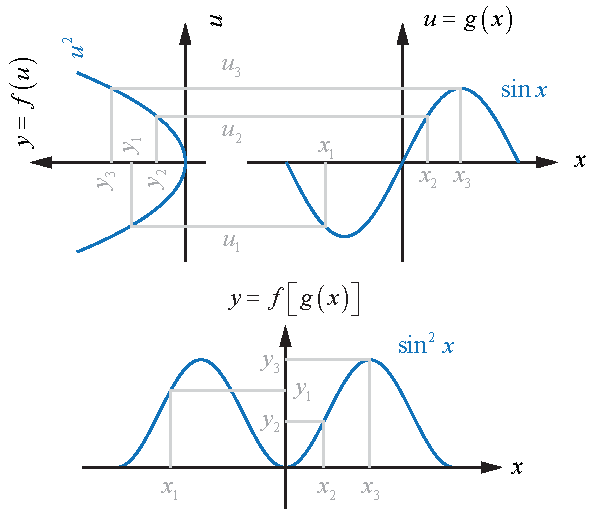
\includegraphics[width=10.5cm]{./figures/ChainR1.pdf}
\caption{可以将 $\sin^2 x$ 看做 $f(u) = u^2$ 和 $g(x) = \sin x$ 的复合函数}\label{ChainR_fig1}
\end{figure}

我们可以用类似\autoref{ChainR_fig1} 的图像来直观地理解复合函数. 先画出 $y = f(u)$ 和 $u = g(x)$ 的图像,并将 $g(u)$ 的图像逆时针旋转 90° 使得两图的 $u$ 轴对齐.这样对于任何定义域中的自变量 $x$, 我们只需要先在 $g(x)$ 的图中画出 $u$ 的位置, 再对应到 $f(u)$ 的图像中求出 $y$ 的位置即可. 

现在我们要讨论的问题是,若已知两函数的导函数 $f'(x)$ 和 $g'(u)$(假设它们在定义域内处处可导)如何求复合函数 $f[g(x)]$ 的导数.

对于给定的 $x$,我们先来看当 $x$ 增加 $\Delta x$ 时 $y$ 的增量 $\Delta y$ 的大小.我们可以使用与\autoref{ChainR_fig1} 类似的方法画出\autoref{ChainR_fig2},然后只需要令 $\Delta x \to 0$, 就可以根据定义求出复合函数的导数
\begin{equation}
f[g(x)]' = \dv{x} f[g(x)] = \lim_{\Delta x\to 0} \frac{\Delta y}{\Delta x}
\end{equation}

\begin{figure}[ht]
\centering
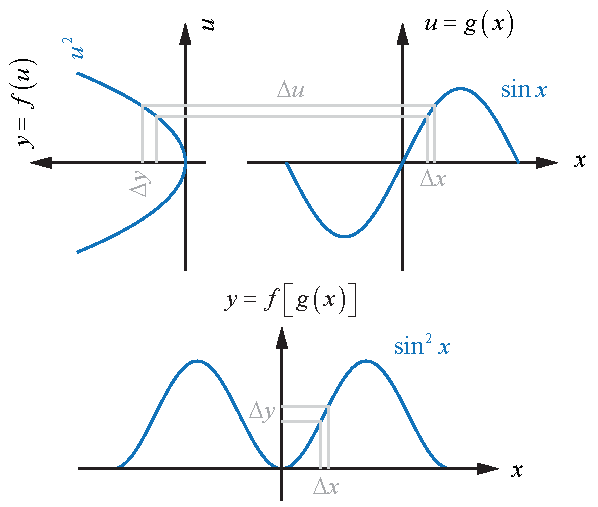
\includegraphics[width=10.5cm]{./figures/ChainR2.pdf}
\caption{用\autoref{ChainR_fig1} 中的方法求出任意 $\Delta x$ 对应的 $\Delta y$} \label{ChainR_fig2}
\end{figure}

在这个过程中,我们在得到 $\Delta y$ 之前先得到了 $u$ 的增量 $\Delta u$. 当 $\Delta x$ 较小时有微分近似(\autoref{Diff_eq2}\upref{Diff})
\begin{equation}
\Delta {u} \approx g'(x) \Delta{x}
\qquad
\Delta{y} \approx f'(u) \Delta{u}
\end{equation}
当 $\Delta x \to 0$ 时对应的微分关系(\autoref{Diff_eq1}\upref{Diff})为
\begin{equation}
\dd{u} = g'(x) \dd{x}
\qquad
\dd{y} = f'(u) \dd{u}
\end{equation}
将上式中的左边代入右边得
\begin{equation}
\dd{y} = f'(u) g'(x) \dd{x} = f'[g(x)]g'(x) \dd{x}
\end{equation}
而复合函数的微分是
\begin{equation}
\dd{y} = f[g(x)]' \dd{x}
\end{equation}
对比以上两式(微分和导数的关系)得
\begin{equation}\label{ChainR_eq4}
f[g(x)]' = f'[g(x)]g'(x)
\end{equation}
这就是复合函数的求导公式.

在上面的例子中 
\begin{equation}
g(x) = \sin x \qquad
g'(x) = \cos x \qquad %链接未完成,引用基本函数求导公式
f(u) = u^2 \qquad
f'(u) = 2u \qquad
\end{equation}
代入上式得
\begin{equation}
\dv{x} \sin^2 x = 2\sin x \cos x
\end{equation}

复合函数的求导公式也叫\bb{链式法则}, 原因是我们可以把以上推导过程用导数的另外一种符号表示如下.
\begin{equation}
\dd{y} = \dv{y}{u} \dd{u} = \dv{y}{u} \dv{u}{x} \dd{x}
\end{equation}
得
\begin{equation}
\dv{y}{x} = \dv{y}{u} \dv{u}{x}
\end{equation}
这种书写方式让人不禁想把 $\dv*{y}{x}$ 看做是 $\dd{y}$ 和 $\dd{x}$ 相除,这样的符号分割是错误的,尤其是在以后学习高阶导数和偏导数时.%链接未完成

\subsection{多重复合函数}
要对多重复合函数如 $f[g(h(x))]$ 求导, 可以先对 $g[h(x)]$ 求导得 $g'[h(x)]h'(x)$ 再得到
\begin{equation}
f[g(h(x))]' = f'[g(h(x))]g'[h(x)]h'(x)
\end{equation}
令 $v = h(x)$, 用微分符号可以表示为
\begin{equation}
\dv{y}{x} = \dv{y}{u}\dv{u}{v}\dv{v}{x}
\end{equation}
任意多重的复合函数求导同理可得.

\phantom{空白行}
\begin{exam}{对函数求导}
\begin{equation}
\frac{1}{\sqrt{x^2+a^2}}
\end{equation}
首先令 $f(x) = 1/\sqrt{x}$ 再令 $g(x) = x^2+a^2$, 上式等于 $f[g(x)]$. 由基本初等函数的导数\upref{FunDer},
\begin{equation}
f'(x) = -\frac{1}{2\sqrt{x^3}}  \qquad g'(x) = 2x
\end{equation}
代入\autoref{ChainR_eq4}, 得
\begin{equation}
\dv{x} \frac{1}{\sqrt{x^2+a^2}} =  f'[g(x)] g'(x) = -\frac{x}{\sqrt{(x^2+a^2)^3}}
\end{equation}
\end{exam}

一种较灵活的情况是,当三个变量只有一个自由度\footnote{即任何一个变量值确定后,另外两个变量也随之确定}时,任何一个变量都可以看做任何另外一个变量的函数\footnote{姑且假设不会出现一个自变量对应两个因变量的情况},这时可以根据需要灵活运用链式法则,如\autoref{ChainR_ex3}.

\begin{exam}{加速运动公式}\label{ChainR_ex3}
假设质点做一维运动,位移,速度和加速度分别为 $x(t)$,  $v(t) = \dv*{x}{t}$,  $a(t) = \dv*{v}{t}$, 但若把速度 $v$ 看做复合函数 $v[x(t)]$, 根据链式法则有
\begin{equation}
a = \dv{v}{t} = \dv{v}{x}\dv{x}{t} = \dv{v}{x}v
\end{equation}
写成微分表达式,有 $a\dd{x} = v\dd{v}$. 注意到 $\dd (v^2) = 2v\dd{v}$, 代入得
\begin{equation}
\dd(v^2) = 2a \dd{x}
\end{equation}
若质点做匀加速运动,该式的物理意义是在任何一段微小时间内,速度平方的增量正比于这段时间内的位移增量.在一段时间 $[t_1,t_2]$ 内把这些增量累加起来,就得到高中熟悉的运动学公式
\begin{equation}
v_2^2-v_1^2 = 2a(x_2-x_1)
\end{equation}
其中 $x_1,v_1$ 和 $x_1,v_1$ 分别是 $t_1,t_2$ 时刻的位置和速度.
\end{exam}
